\section{ارتباط بین دو آردوینو با استفاده از پروتکل \lr{SPI}}

\subsection{اهداف آزمایش}
\begin{itemize}
    \item آشنایی با پروتکل ارتباطی \lr{SPI}
    \item آشنایی با پروتکل سریال و ارتباط با کامپیوتر از طریق آن
\end{itemize}

\subsection{قطعات مورد نیاز}
\begin{itemize}
    \item \lr{Arduino Uno}
    \item صفحه نمایش \lr{LCD}
    \item پتانسیومتر ۱ کیلواهم \lr{B1K}
    \item مقاومت ۲۲۰ اهم

\end{itemize}

\subsection{مقدمه}
تا اینجا آردوینوی ما ارتباطی با کامپیوتری که از طریق آن برنامه ها را روی آن آپلود می‌کردیم نداشت. می‌توانیم با استفاده از ارتباط سریال، این کار را انجام دهیم. برای این کار کافیست از کتاب‌خانه‌ی سریال استفاده کنیم.
\newline
\textcolor{red}{\begin{nas}سوال: \end{nas}}
در مستندات آردوینو جست‌و‌جو کنید و در مورد توابع کتاب‌خانه‌ی \lr{Serial} توضیح دهید.
\newline
با پروتکل \lr{SPI} در درس ریزپردازنده آشنا شدید.
همانطور که می‌دانید این نوع ارتباط از نوع ارتباطات \lr{Master\Slave} است. در این نوع ارتباطات یک دستگاه می‌تواند با چند دستگاه دیگر ارتباط برقرار کند. در ارتباط \lr{SPI} بورد مرکزی یا همان \lr{Master} بوردی که میخواهد با آن ارتباط برقرار کند را انتخاب کرده و برای آن پیامی ارسال می‌کند و در صورت نیاز، از آن درخواست پاسخ می‌کند.
\newline
\textcolor{red}{\begin{nas}سوال: \end{nas}}
در مورد پروتکل \lr{SPI} به سوالات یر پاسخ دهید:
\begin{itemize}
    \item این پروتوکل از ۴ سیم استفاده می‌کند. وظیفه‌ی هر یک از این ۴ سیم را شرح دهید.
    \item آیا این پروتکل امکان حضور چند \lr{Master} را به ما می‌دهد؟
    \item در بورد \lr{Arduino Uno} کدام پین های به صورت پیش‌فرض برای پین های \lr{SPI} تخصیص داده شده‌اند؟
    \item در این پروتکل ارتباطی سنکرون، کلاک توسط \lr{Master} تعیین می‌شود یا \lr{Slave}؟
\end{itemize}
\newline
می‌توانیم برای استفاده از این پروتکل، از کتابخانه‌ی \lr{SPI.h} استفاده کنیم. این کتاب‌خانه یک لایه‌ی انتزاع برای ارتباط با سخت‌افزار مخصوص \lr{SPI} در میکروکنترلر های مختلف است و این اجازه را به ما می‌دهد که به صورت نسبتا \lr{Portable} برنامه‌ای بنویسیم که از این کتاب‌خانه استفاده کند.
\newline
\textcolor{red}{\begin{nas}سوال: \end{nas}}
در مستندات این کتاب‌خانه جستوجو کنید و در مورد توابع زیر توضیح بدهید:
\begin{itemize}
    \item \lr{SPI.begin()}
    \item \lr{SPI.beginTransaction()}
    \item \lr{SPI.end()}
    \item \lr{SPI.transfer()}
    \item \lr{SPI.usingInterrupt()}
\end{itemize}
در این آزمایش باید آردوینوی ما هم در حالت \lr{Master} و هم در حالت \lr{Slave} کار کند.
\newline
\textcolor{red}{\begin{nas}سوال: \end{nas}}
دستوری که با استفاده از آن آردوینو در حالت \lr{Slave} قرار می‌گیرد را بنویسید و آن را توضیح دهید.

\subsection{شرح آزمایش}

می‌خواهیم یک برنامه‌ی گفت‌وگو با معماری \lr{Client/Server} درست کنیم. برنامه‌ی کلاینت باید یک پیام به برنامه‌ی سرور بدهد و برنامه‌ی سرور نیز این پیام را به همه مخابره کند. شما باید هر دو برنامه های کلاینت و سرور را درست کنید و با کمک همکلاسی هایتان آن را آزمایش کنید. به این صورت که برای تست کردن برنامه‌ی سرور خود، یک یا چند گروه دیگر برنامه‌ی کلاینتشان را به شما متصل می‌کنند و آنها همزمان برنامه‌ی خودشان را تست می‌کنند. به همین صورت نیز شما برنامه‌ی کلاینت خود را تست خواهید کرد. توجه کنید در صورتی که به دلیل مشکل در سرور/کلاینت گروه دیگر برنامه‌ی کلاینت/سرور شما خروجی صحیح نداد به شما نیز نمره‌ی آزمایش تعلق نخواهد گرفت پس به یک دیگر کمک کنید. طبیعتا اعضای هر گروه باید بتوانند که برنامه های گروه خود را به طور کامل توضیح بدهند.
\newline

از آنجایی که برنامه های شما بین گروه های مختلف باید کارکرد داشته باشد، به یک پروتکل ارتباطی سطح کاربرد نیز نیاز داریم. برای همین همه‌ی گروه ها باید از این الگوریتم در برنامه‌ های کلاینت و سرور خود استفاده کنند.

\subsubsection{الگوریتم سرور}
\begin{enumerate}
    \item سرور هر ۱ ثانیه یک بار با هر کلاینت ارتباط برقرار می‌کند تا ببیند پیامی برای مخابره دارد یا نه. در این مخابره، سرور بایت اول صفر را برای کلاینت می‌فرستد.
    \item در صورت داشتن پیام، پیامی که صورت یک رشته مانند رشته های \lr{C} است را دریافت می‌کند. منظور از رشته های مانند \lr{C} این است که پایان رشته را یک بایت صفر نشان می‌دهد.
    \item .رشته را روی صفحه نمایش نمایش می‌دهد
    \item رشته را برای همه‌ی کلاینت ها مخابره می‌کند. در این مخابره، سرور بایت اول ۱ را برای کلاینت می‌فرستد و سپس ارسال رشته را شروع می‌کند.
\end{enumerate}


\subsubsection{الگوریتم کلاینت}
\begin{enumerate}
    \item کلاینت منتظر است تا سرور با آن ارتباط برقرار کند. و همچنین از طریق کامپیوتر و با استفاده از کتاب‌خانه‌ی \lr{Serial} از کاربر ورودی می‌گیرد.
    \item ورودی گرفته شده از کاربر در یک بافر ذخیره می‌شود.
    \item پس از برقراری ارتباط، در صورتی که بایت صفر دریافت کرد محتویات بافر را برای سرور می‌فرستد.
    \item در صورتی که بایت یک دریافت کرد یعنی سرور می‌خواهد برای ما پیام بفرستد. پس از دریافت پیام، کلاینت آن را روی صفحه نمایش نشان می‌دهد.
\end{enumerate}

توجه داشته باشید که دستگاه \lr{Slave} حتما باید در حالت \lr{Slave} قرار بگیرند. در غیر این صورت هر دو دستگاه می‌خواهند کلاک را خودشان تامین کنند و احتمال خرابی قطعات وجود دارد. می‌توانید برای اطلاعات بیشتر به
\href{https://circuitdigest.com/microcontroller-projects/arduino-spi-communication-tutorial}{این لینک}
مراجعه کنید.

\newline
\begin{figure}[h]
    \centering
    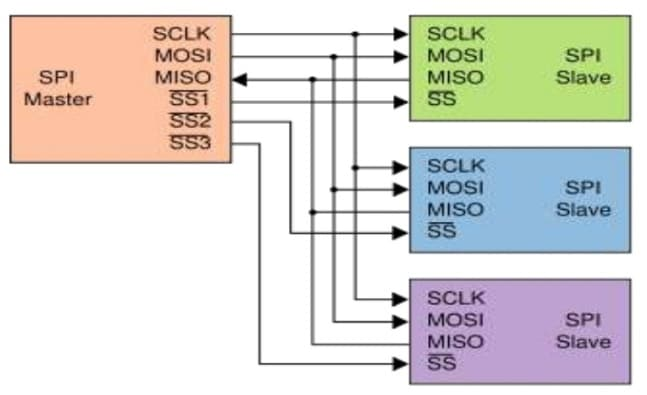
\includegraphics[width=8cm]{SPI_BUS.jpg}
    \caption{یک نمونه از باس \lr{SPI}}
    \label{fig:spibus}
\end{figure}
\newline